Apvienoto Nāciju Organizācijas Klimata konferencē Parīzē 2015. gada decembrī daudzas pasaules valstis vienojās ierobežot globālo sasilšanu zem 2\textdegree C salīdzinājumā ar pirmsindustriālo laikmetu.
%, tāpēc ES ir apņēmusies līdz 2030. gadam samazināt siltumnīcefekta gāzu emisijas vismaz par 40\% salīdzinājumā ar 1990. gada līmeni.
Tāpēc Eiropas Savienībā noteikts dalībvalstīm saistošs mērķrādītājs  –  vismaz 32\%  atjaunojamās enerģijas īpatsvars līdz 2030. gadam \cite{ES}.

Ne mazāk būtiska ir atjaunojamo energoresursu loma energoapgādes neatkarības un drošības veicināšanā, tehnoloģiju attīstībā un inovācijās, vienlaikus sniedzot labumu videi un sabiedrībai, kā arī nodrošinot svarīgus priekšnosacījums nodarbinātībai, reģionālajai attīstībai un elektrības nodrošināšanai grūti pieejamās vietās \cite{ES}.

Dažādu atjaunojamo enerģijas resursu - saules, vēja, ģeotermālo un ūdens - starpā Saules enerģija ir viens no kandidātiem klimata pārmaiņu un to seku mazināšanai un efektīvas energoapgādes nodrošināšanai. Pēdējā desmitgadē veiktās investīcijas Saules enerģijas izmantošanā manifestējās inovācijās saules paneļu ražošanā, un gala rezultātā tie ir kļuvuši efektīvāki un finansiāli pieejamāki patērētājiem, piemēram, silīcija saules paneļu cena sastāda mazāk nekā 30\% no kopējām saules paneļu sistēmas uzstādīšanas izmaksām un to saražotā enerģija atmaksājas vidēji trīs gadu periodā \cite{researchOpp}. Tomēr bez klimata to efektivitāti ietekmē arī daudzi citi faktori, kas tiek analizēti šajā darbā, piemēram, saules paneļu tips un telpiskā orientācija.

Šī pētījuma \textbf{mērķis} ir analizēt un praktiski pārbaudīt divu tipu (JA un LG) saules paneļu efektivitāti atšķirīgos telpiskās orientācijās risinājumos -- pētītas trīs dažādu virzienu (dienvidu (D), rietumu (R), austrumu (A)) un trīs leņķu pret horizontu (13\textdegree, 40\textdegree, 90\textdegree) paneļu grupas -- un tiek salīdzināta to piemērotība Latvijas klimatiskajiem apstākļiem.

% \subsection{Darba uzdevumi}
\textbf{Darba uzdevumi}
\begin{itemize}
\item Ievākt, atlasīt un analizēt saules paneļu jaudas (P) datus.
\item Izveidot iespējami automatizētu datu apstrādes sistēmu R valodā ilgtermiņa montioringa vajadzībām.
\item Salīdzināt paneļu efektivitāti gada laikā mēnešu intervālos atbilstoši tipa un telpiskās orientācijas apakšgrupām.
% \item Balstoties uz ilgtermiņa saules izstarojuma monitoringu, novērtēt saules paneļu saražoto enerģiju no fizikālajiem apsvērumiem.
\item Novērtēt datu kvalitāti no fizikālo apsvērumu un saules apstarojuma mērījumu viedokļa.
\end{itemize}

% \subsection{Darba aktualitāte}
\textbf{Darba aktualitāte}

Darba nozīme atklājas detalizētas paneļu efektivitātes analīze nepieciešamībā tieši Latvijas klimatiskajiem apstākļiem. Latvijā veikto pētījumu daudzums un kvalitāte pagaidām neļauj iegūt pilnīgu priekšstatu par Saules paneļu lietošanas iespējām un prognozēt dažādu paneļu tipu efektivitāti reālā Latvijas klimatā. Tāpēc šī darba novitāte ietverta programmatūras izveidē, kas ļauj attēlot un apstrādāt Saules paneļu monitoringa datus, kas dos iespēju veikt turpmākus dziļākus pētījumus par dažādiem saules paneļu spēkstaciju pielietojuma aspektiem Latvijā.\\
% \subsection{Darba struktūra}

\textbf{Darba struktūra}

Darba pirmo daļu veido literatūrā pieejamo Saules apstarojuma novērtējumu raksturojums un apskats par Saules redzamo pārvietošanās pie debess sfēras diennakts laikā 60 dienu intervālos. Otrajā daļā aplūkota saules paneļu uzbūve un to darbības princips. Trešajā daļā tiek apskatīta saules paneļu sistēmas elektriskā shēma un raksturoti LU Botāniskā dārza spēkstacijas instalācijas parametri.
Ceturtajā daļā ir aprakstīti iegūtie rezultāti, tie ir salīdzināti savā starpā, ar citas saules paneļu spēkstacijas mērījumu rezultātiem, ar eksperimentālā poligona meteostacijas datiem par solāro apstarojumu šajā laika periodā, kā arī aplūkoti no teorētiskās pusvadītāju fizikas aspektiem.\\

\textbf{Autores ieguldījums darbā}
% \subsection{Autores ieguldījums darbā}
% the \\ insures the section title is centered below the phrase: Appendix B

Saules paneļu uzstādīšanu veica SIA EG Inženieri Valda Gailīša vadībā.
Par datu ievākšanu no saules paneļu sistēmas datu uzkrājējiem jāpateicas Victron Energy B.V. izstrādātājai VRM sistēmai.

Mans ieguldījums ir koda arhitektūras plānošana, rakstīšana un uzturēšana līdz šim brīdim. Esmu vienīgais koda bāzes izstrādātājs. Darbā kopā veikti 318 iesūtījumi (\textit{commits}) trīs zaros (105, 123 un 90 iesūtījumi attiecīgi), kas rezultējās 3140 koda rindās. 

Darba gaitā veicu datu lejupielādi, datu informācijas aptveršanu, kā arī datu programmatisku atlasīšanu, apstrādi, apkopošanu, transformēšanu vizualizācijas vajadzību pielāgošanai un datu vizualizāciju. 

% \begin{figure}[h]
% 	\centering
% 	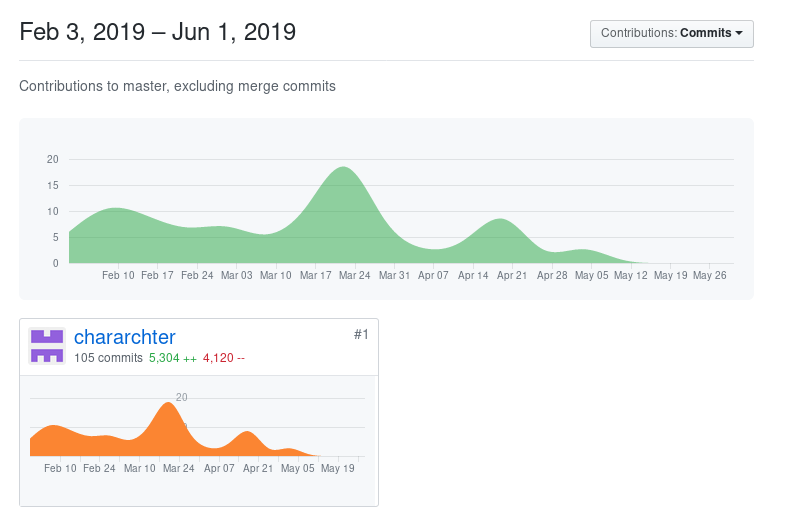
\includegraphics[width=0.6\linewidth]{figures/misc/contributions.png}
% 	\caption{Darba autores ieguldījums master zarā.}
% 	\label{fig:retribution}
% \end{figure}